% !TEX program = pdflatex
%
% Nokor Pass: Repeat Visits, Not Promotion
% A National Visitor Substrate for Cambodia's Tourism Recovery
% Preprint. Comments welcome.
%
% Build: latexmk -pdf main.tex

\documentclass[10pt,letterpaper,twocolumn]{article}

\usepackage[T1]{fontenc}
\usepackage[utf8]{inputenc}
\usepackage{mathptmx}
\usepackage[scaled=0.92]{helvet}
\usepackage{courier}
\usepackage{textcomp}
\usepackage[top=0.9in,bottom=0.9in,left=0.85in,right=0.85in]{geometry}
\setlength{\columnsep}{0.3in}
\usepackage[protrusion=true,expansion=false]{microtype}
\usepackage{graphicx}
\usepackage{booktabs}
\usepackage{tabularx}
\usepackage{array}
\usepackage{enumitem}
\usepackage[authoryear,round]{natbib}
\usepackage{titlesec}
\usepackage{fancyhdr}
\usepackage[font=small,labelfont=bf,labelsep=period]{caption}
\usepackage{xcolor}
\usepackage[hyphens]{url}
\usepackage[hidelinks,breaklinks]{hyperref}

% Long URLs in references must break inside a two-column measure.
\makeatletter
\g@addto@macro\UrlBreaks{%
  \do\a\do\b\do\c\do\d\do\e\do\f\do\g\do\h\do\i\do\j\do\k\do\l\do\m%
  \do\n\do\o\do\p\do\q\do\r\do\s\do\t\do\u\do\v\do\w\do\x\do\y\do\z%
  \do\0\do\1\do\2\do\3\do\4\do\5\do\6\do\7\do\8\do\9\do\-\do\.\do\=\do\&\do\?}
\makeatother
\Urlmuskip=0mu plus 1mu
\setlength{\emergencystretch}{3em}
\tolerance=1200

\hypersetup{
  pdftitle={Nokor Pass: Repeat Visits, Not Promotion},
  pdfauthor={Sengtha Chay, Langdy Khut, Mouniseyhak Va},
  pdfsubject={A national visitor substrate for Cambodia's tourism recovery},
  pdfkeywords={tourism recovery, repeat visitation, word of mouth, destination image, payments, Cambodia},
}

% Headings in the style of the CamboVerse preprints: "1. Introduction", "1.1 ...".
\titleformat{\section}{\normalfont\large\bfseries}{\thesection.}{0.5em}{}
\titleformat{\subsection}{\normalfont\normalsize\bfseries}{\thesubsection}{0.6em}{}
\titlespacing*{\section}{0pt}{1.6ex plus .4ex minus .2ex}{0.9ex}
\titlespacing*{\subsection}{0pt}{1.3ex plus .3ex minus .2ex}{0.6ex}

% Running head and page number.
\pagestyle{fancy}
\fancyhf{}
\fancyhead[L]{\small\itshape Nokor Pass --- Repeat Visits, Not Promotion}
\fancyfoot[C]{\small\thepage}
\renewcommand{\headrulewidth}{0.4pt}
\fancypagestyle{plain}{%
  \fancyhf{}%
  \fancyhead[L]{\small\itshape Nokor Pass --- Repeat Visits, Not Promotion}%
  \fancyfoot[C]{\small\thepage}%
  \renewcommand{\headrulewidth}{0.4pt}}

\setlist{leftmargin=1.2em,itemsep=0.2em,topsep=0.3em}
\renewcommand{\arraystretch}{1.15}
\newcolumntype{L}{>{\raggedright\arraybackslash}X}

% Run-in paragraph labels.
\newcommand{\runin}[1]{\textbf{#1}\quad}

\title{\Large Nokor Pass: Repeat Visits, Not Promotion\\[0.3em]
  \large A National Visitor Substrate for Cambodia's Tourism Recovery}

\author{%
  Sengtha Chay\textsuperscript{1}\qquad Langdy Khut\textsuperscript{2}\qquad Mouniseyhak Va\textsuperscript{2}\\[0.6em]
  \normalsize National University of Management, Phnom Penh, Cambodia\\[0.6em]
  \small\textsuperscript{1}Director, CamboVerse Center\qquad \textsuperscript{2}CamboVerse DevOps\\[0.6em]
  \small Corresponding author: \texttt{sengtha@num.edu.kh}}

\date{\normalsize October 2026\\[0.2em]\emph{Preprint --- comments welcome.}}

\begin{document}

\twocolumn[
  \begin{@twocolumnfalse}
    \maketitle
    \vspace{0.5em}
  \end{@twocolumnfalse}
]
\thispagestyle{plain}

{\small
\noindent\textbf{Keywords:} tourism recovery; repeat visitation; destination
loyalty; word of mouth; destination image; tourist payments; soulbound
credentials; purpose-bound money; Cambodia; CamboVerse

\smallskip
\noindent\textbf{JEL classification:} Z32; Z38; E42; O33; L86

\medskip
\noindent\textbf{Disclaimer}\par
\noindent This is independent academic research. The views are the authors' own
and do not represent the National University of Management or any body within
it.

The paper is not affiliated with, endorsed by, funded by, commissioned by, or
developed for any government, ministry, central bank, heritage authority or
other institution. Institutional roles named in the design --- issuer, operator,
site authority --- are proposals; nothing here implies adoption by, or a mandate
for, any body. Nokor Pass, kRIEL, kUSD and Nokor Point are names proposed in this
paper. CamboVerse is a project name and the CamboVerse Center is an institute
appearing only as the authors' affiliation.

Nothing described here has been deployed or trialled, and no visitor data has
been collected.

\medskip
\noindent\textbf{Abstract}\par
\noindent Cambodia received 5.57 million international visitors in 2025, 16.9\%
fewer than in 2024, and arrivals fell a further 44.4\% in the first eight months
of 2026. Neighbouring Vietnam grew in the same years under the same fuel prices
and regional tension. The usual response to a fall like this is promotion. We
argue that promotion cannot repair a destination whose image has been damaged,
because a reader who has seen headlines about scam compounds does not believe
an advertisement. What repairs an image is the testimony of people who went,
and that testimony accumulates only through visits that go well and visitors
who come back or send others.

We propose Nokor Pass, a national visitor substrate on the Base blockchain, as
the instrument that makes this strategy work and makes it measurable. It has
four parts: a soulbound pass issued at arrival and bound to existing identity
checks; riel and dollar tokens (kRIEL, kUSD) used for every payment, with
merchant-initiated requests, a dispute window, and cash-out only through an
operator; the pass as the access ticket to every heritage site; and conversion
back to cash at departure. A separate, giftable Nokor Point records word of
mouth as points earned on one trip and spent on a later one, or by someone
else. CamboVerse, an open virtual Cambodia, exposes the lesser-known sites the
pass then opens.

The paper makes no empirical claim. Nothing has been deployed. Every
substantive statement is classed as specified, carried, analytic or
conjectural, and we state what the design does not solve: the reputation damage
itself, the border conflict, and global demand. The design requires the state
to act, and we name the institutional changes it depends on.
\par}

% ---------------------------------------------------------------------------
\section{Introduction}
\label{sec:intro}

Cambodia's foreign arrivals have halved in two years. The Ministry of Tourism
recorded 6.7 million international visitors in 2024 and 5.57 million in 2025
\citep{cir2026}. In the first eight months of 2026 it recorded 2.25 million,
against 4.05 million in the same months of 2025 \citep{khmertimes2026}. Foreign
visitors to the Angkor Archaeological Park fell 29\% over the same eight months
\citep{peninsula2026}.

The Ministry names the causes: publicity about online scam compounds, the
conflict on the Thai border, and higher fuel prices \citep{thestar2026}.
Overland arrivals from Thailand fell 96\% between January and May 2026
\citep{nomadlawyer2026}. Yet Vietnam, facing the same fuel prices and the same
regional tension, received a record 21.2 million visitors in 2025 and grew a
further 14.4\% in the first eight months of 2026 \citep{wikivn,vnat2026}. The
external shocks are real, but they do not explain the gap.

The response these figures usually provoke is promotion: campaigns, roadshows,
visa waivers for one market. We argue this misreads the problem. A destination
whose image has been damaged by news reports is not short of awareness. It is
short of belief. A person who has read about scam compounds does not believe an
advertisement saying Cambodia is safe; they believe a friend who went.
Promotion can amplify a reputation, but it cannot create one.

\subsection{What we claim}

\runin{First: the lever is visitors' experience.} The lever that repairs a
damaged image is the accumulated experience of visitors, carried home as word of
mouth. Its unit is not a new arrival but a returning one, or one sent by a
previous visitor. We draw this from tourism research on revisit intention and
from four national cases: Japan, Vietnam, Singapore and Colombia.

\runin{Second: that lever needs an instrument.} Repeat visits and word of mouth
cannot be managed if they cannot be measured, and they will not grow while
visitors are cheated in the transactions that make up a trip. Cambodia currently
measures arrivals, not returns, and its dominant payment rail, KHQR, leaves
visitors exposed to fraud they cannot see.

\runin{Third: we specify that instrument.} Nokor Pass is a national visitor
substrate with four functions: identity, payment, site access and departure
refund. A separate, giftable Nokor Point turns word of mouth into something that
can be counted. CamboVerse, an open virtual Cambodia built at our university,
exposes the lesser-known sites the pass then opens.

\runin{Fourth: only the state can build it.} The instrument requires
immigration, the central bank, the tourism ministry and the site authorities to
act together, and we name what each must change.

Section~\ref{sec:related} reviews prior work. Section~\ref{sec:method} sets out
our method. Section~\ref{sec:cases} reads the four national cases.
Section~\ref{sec:design} describes the design, and Section~\ref{sec:follows}
works out what follows from it. Section~\ref{sec:institutions} lists the
institutional changes required. Sections~\ref{sec:notsolve}
and~\ref{sec:unknown} state what the design does not solve and what we do not
know. Section~\ref{sec:next} sets out next steps, and
Section~\ref{sec:conclusion} concludes.

% ---------------------------------------------------------------------------
\section{Related Work}
\label{sec:related}

Four bodies of work bear on this paper. None of them joins tourism loyalty to
payment design, which is the gap we address.

\subsection{Revisit intention and destination loyalty}

Tourism research treats loyalty as two behaviours: returning, and
recommending. \citet{oppermann2000} argued that destination loyalty should be
measured over a visitor's travel history, not a single trip.
\citet{yoon2005} modelled loyalty as driven by motivation through satisfaction.
\citet{chi2008} found that destination image shapes satisfaction, and that both
shape loyalty, with satisfaction mediating part of image's effect. The common
thread is that what a visitor experienced predicts whether they return and what
they say. We carry this finding; we do not test it.

\subsection{Word of mouth}

\citet{litvin2008} showed that electronic word of mouth had become a principal
channel through which travellers judge destinations. Advertising surveys have
long found that recommendations from people one knows are trusted above any
paid message \citep{nielsen2015}. For a damaged destination this matters twice:
the negative stories already circulate this way, so the corrective must travel
the same way.

\subsection{Recovering a damaged image}

Places in crisis have tried many media strategies \citep{avraham2008}.
Colombia's 2008 campaign, \emph{Colombia, the only risk is wanting to stay}, is
the case most cited for turning a reputation for danger into an invitation.
\citet{fletcher2010} notes that foreign embassies kept warning travellers about
Colombia long after the campaign began. The campaign's slogan stated a claim;
visitors' experiences were what made it believable. We return to this in
Section~\ref{sec:colombia}.

\subsection{Tourist payments and purpose-bound money}

Three recent schemes are close to our design. Cambodia's own central bank
launched the Bakong Tourists app with Mastercard in November 2024: visitors
verify with a passport and selfie, top up by card, hold dollars or riel, and
pay any KHQR merchant \citep{fintechnews2024}. Thailand opened an 18-month
regulatory sandbox, TouristDigiPay, in August 2025, letting visitors convert
crypto-assets to baht through licensed platforms for local spending
\citep{theblock2025}. Singapore's central bank published a protocol for
purpose-bound money in June 2023, under which digital money can carry
conditions such as a validity period or the types of shop that may accept it
\citep{mas2023}.

None of these schemes addresses the two things our argument needs. They make
paying easier, but the payee still receives liquid money on a final rail, so
the fraud exposure described in Section~\ref{sec:payments} remains. And none is
built to measure whether visitors return or send others.

% ---------------------------------------------------------------------------
\section{Method}
\label{sec:method}

\subsection{What kind of paper this is}

This is a design proposal, not an evaluation. It diagnoses a policy problem
from published data, reads four national cases for what they suggest, specifies
an instrument, and works out what follows from its rules. Nothing in it has
been deployed or measured. The design is normative in one further sense: it
assumes the state is willing to change the rules that would currently prevent
it, and Section~\ref{sec:institutions} lists those rules.

\subsection{Four kinds of claim}

Every substantive statement in this paper is one of four kinds, and we keep
them apart, following \citet{chay2026precinct}.

\begin{itemize}
  \item A \textbf{specified} claim is true of the design as written in
  Section~\ref{sec:design} and in its published specification, and can be
  checked against them.
  \item A \textbf{carried} claim is established elsewhere and imported:
  published statistics, prior research, official documents.
  \item An \textbf{analytic} claim follows logically from stated premises. It
  is not an empirical finding, but given its premises it holds.
  \item A \textbf{conjectural} claim is a reasoned expectation about how people
  or institutions will behave. Nothing here establishes it; it is offered to be
  tested.
\end{itemize}

The line most easily blurred to our advantage is the one between analytic and
conjectural, so we state it sharply with an example. That a merchant who
receives a claim redeemable only through an operator cannot withdraw the
proceeds of a disputed payment before the dispute window closes is analytic: it
follows from the rules. That fewer merchants will then attempt to cheat visitors
is conjectural: it is a claim about behaviour, and we have observed none.

\subsection{Sources}

Arrival, spending and site figures are taken from Cambodia's Ministry of
Tourism and Angkor Enterprise as reported in 2025 and 2026, and from the
national tourism authorities of Vietnam, Japan and Singapore. Several were
found first in news reports; where a primary release was available we cite it,
and where it was not we say so. Survey findings on why visitors return are
carried from published studies and industry surveys, and we state their limits
where we use them.

\subsection{Who we are}

The authors work at the National University of Management in Phnom Penh, where
the CamboVerse Center builds the open virtual Cambodia described in
Section~\ref{sec:camboverse} and would build the reference implementation of
Nokor Pass. We therefore have an interest in the design being adopted. The
reader should weigh our claims with that in mind, and the four-way
classification is meant to make that weighing possible.

% ---------------------------------------------------------------------------
\section{Evidence from Other Countries}
\label{sec:cases}

All four cases point the same way: visitors return and recommend because of
what they experienced, and the levers that work follow experience rather than
precede it. Each case is carried evidence, read for what it suggests; none was
designed as a test of our argument.

\subsection{Japan: past experience is the strongest motive}

Japan's arrivals rose from about 10.4 million in 2013 to 31.9 million in 2019,
after visa waivers for Thailand and Malaysia in 2013 and easier visas for
Chinese visitors \citep{visitinsidejapan2025}. The weak yen is usually credited
for the later boom. Dentsu's Japan Brand Survey, of 12,400 respondents in 20
markets, found instead that the strongest motive for visiting was a previous
visit, and that outside Hong Kong and Taiwan the weak yen was not the main
reason \citep{dentsu2025}. In 2025, 52.7\% said they wanted to visit Japan
again, first among the 20 markets polled \citep{travelvoice2025}.

Japan raised its departure tax from \textyen1,000 to \textyen3,000 in July 2026,
raised visa fees for the first time since 1978, and legislated a pre-travel
authorisation for visa-exempt visitors. Analysts expect little effect on demand
because so many visitors are returning ones \citep{cnbc2026}. The order
matters: Japan opened entry, built a reason to return, and only then charged
for access.

\subsection{Vietnam: the gap opened before the current shocks}

Vietnam's lead over Cambodia opened between 2015 and 2019
(Figure~\ref{fig:arrivals}), before the scam-compound reports and the border
conflict. Those events deepened Cambodia's fall; they cannot explain the gap.

\begin{figure*}[t]
  \centering
  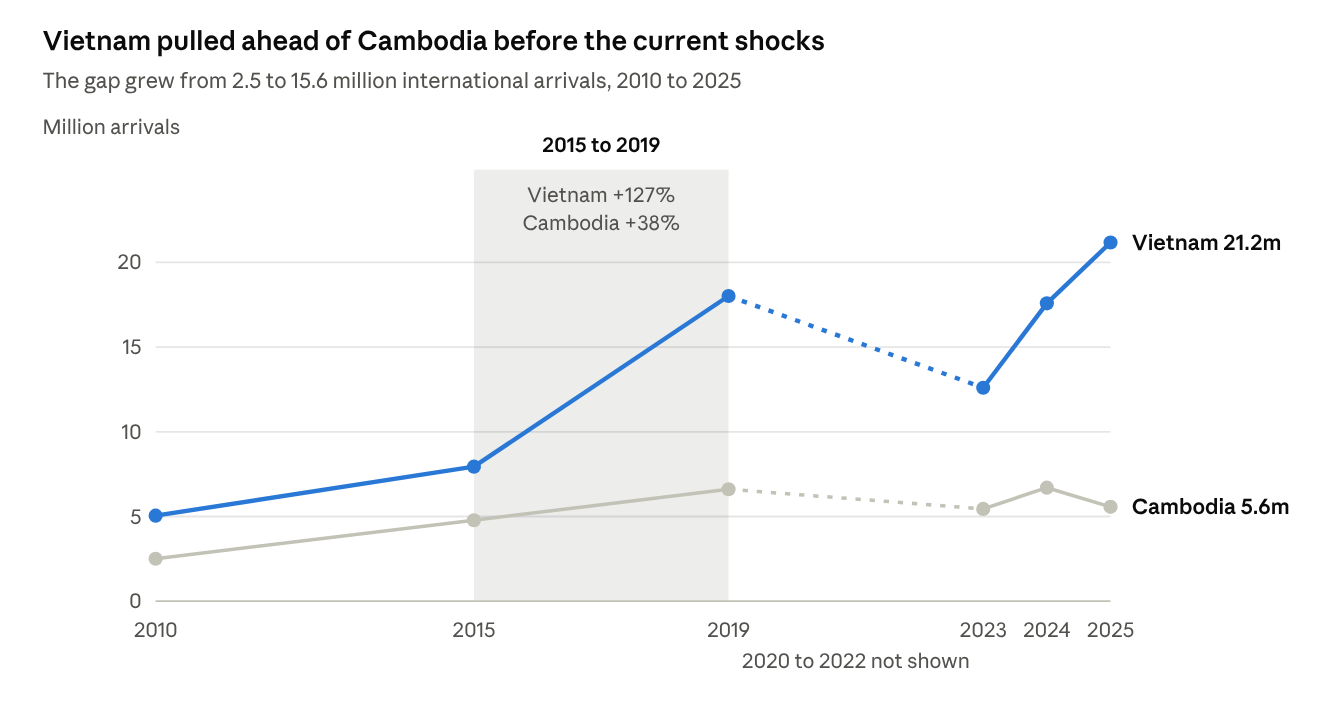
\includegraphics[width=0.82\textwidth]{figures/arrivals.png}
  \caption{International arrivals to Vietnam and Cambodia, 2010--2025, in
  millions. Pandemic years 2020--2022 are not shown. Sources: Ministry of
  Tourism (Cambodia) and Ministry of Culture, Sports and Tourism (Vietnam), as
  tabulated in \citet{wikikh} and \citet{wikivn}.}
  \label{fig:arrivals}
\end{figure*}

Vietnam did not buy this growth with advertising. In 2019 its national tourism
promotion budget was reported at about US\$2 million, 2.9\% of Thailand's
\citep{vnexpress2019}. What it offered instead was several distinct regions to
return to, private investment in attractions that visitors photograph and
share, and food that became a reason to come back. A pre-pandemic national
survey found that 33\% of international visitors were on a second or later
visit and that over 94\% rated their experience good or very good
\citep{saigoneer}. That survey is old, and we cite it as indicative only.

\subsection{Singapore: the brand is the result, not the cause}

Singapore has almost no natural or ancient heritage, yet it received 16.9
million visitors in 2025 and a record S\$32.8 billion in tourism receipts
\citep{stb2026,asiaone2026}. Its arrivals jumped 20\% in 2010, the year two
integrated resorts opened, though the same year saw recovery from the global
recession \citep{lvs2010,asgam2015}. Singapore ranks 21st in Brand Finance's
2026 Global Soft Power Index, first in ASEAN, with its strongest scores in
governance, integrity and safety \citep{brandfinance2026}.

Its 2017 campaign, \emph{Passion Made Possible}, was criticised at launch for
lacking a clear message \citep{comms8_2018}, and arrivals after it grew only
modestly. The reputation that draws visitors to Singapore is not the slogan's
work. It is the accumulated experience of a place where visitors are not
cheated.

\subsection{Colombia: a claim made believable by visitors}
\label{sec:colombia}

Colombia's campaign confronted its reputation for danger directly and has been
credited with rising arrivals and investment. Its own officials said the word
\emph{risk} was used because it was already attached to the country
\citep{colombiareports2011}. But embassies kept warning travellers, and the
slogan could not change their warnings \citep{fletcher2010}. What changed
perception was the stream of visitors who went and reported that the country
was unlike the news. Colombia is the closest analogue to Cambodia's present
problem, and it shows the limit of promotion: a campaign can invite people to
test a claim, but only their experience can confirm it.

\subsection{What the cases share}

Table~\ref{tab:cases} sets the four cases side by side. The reading we take
forward is conjectural for Cambodia, but consistent across four different
countries: experience comes first, and the stories visitors carry home are what
change a destination's image.

\begin{table}[t]
  \centering
  \small
  \caption{What drove visitors in four national cases, and what promotion did.}
  \label{tab:cases}
  \begin{tabularx}{\columnwidth}{@{}p{0.17\columnwidth}LL@{}}
    \toprule
    Case & What drove visitors & What promotion did \\
    \midrule
    Japan & Previous visits; experience and culture & Followed demand; Japan now charges for access \\
    Vietnam & Regions to return to; attractions people share; food & Very little; the budget was small \\
    Singapore & Trust built on safety and governance; created attractions & Amplified an existing reputation \\
    Colombia & Visitors reporting a country unlike the news & Invited people to test the claim \\
    \bottomrule
  \end{tabularx}
\end{table}

% ---------------------------------------------------------------------------
\section{The Design}
\label{sec:design}

All claims in this section are specified: they describe the design as written,
and a reference implementation will be published against them.

\subsection{Overview}

Nokor Pass is one pass for everyone in Cambodia, visitors and residents alike,
held in a phone wallet that never shows the user a seed phrase, a gas fee or a
blockchain. It does four things: it identifies the holder, it pays, it opens
sites, and for visitors it refunds what is left at departure. A separate token,
Nokor Point, records value that can be given to others. CamboVerse, an open
virtual Cambodia, shows the sites the pass opens. Each public body keeps the
role it already has.

Figure~\ref{fig:architecture} shows the arrangement. Each institution issues
one thing into the wallet; each thing is used at one place. The operator runs
escrow and cash-out, and every event feeds the indicators in
Section~\ref{sec:measure}.

\begin{figure*}[t]
  \centering
  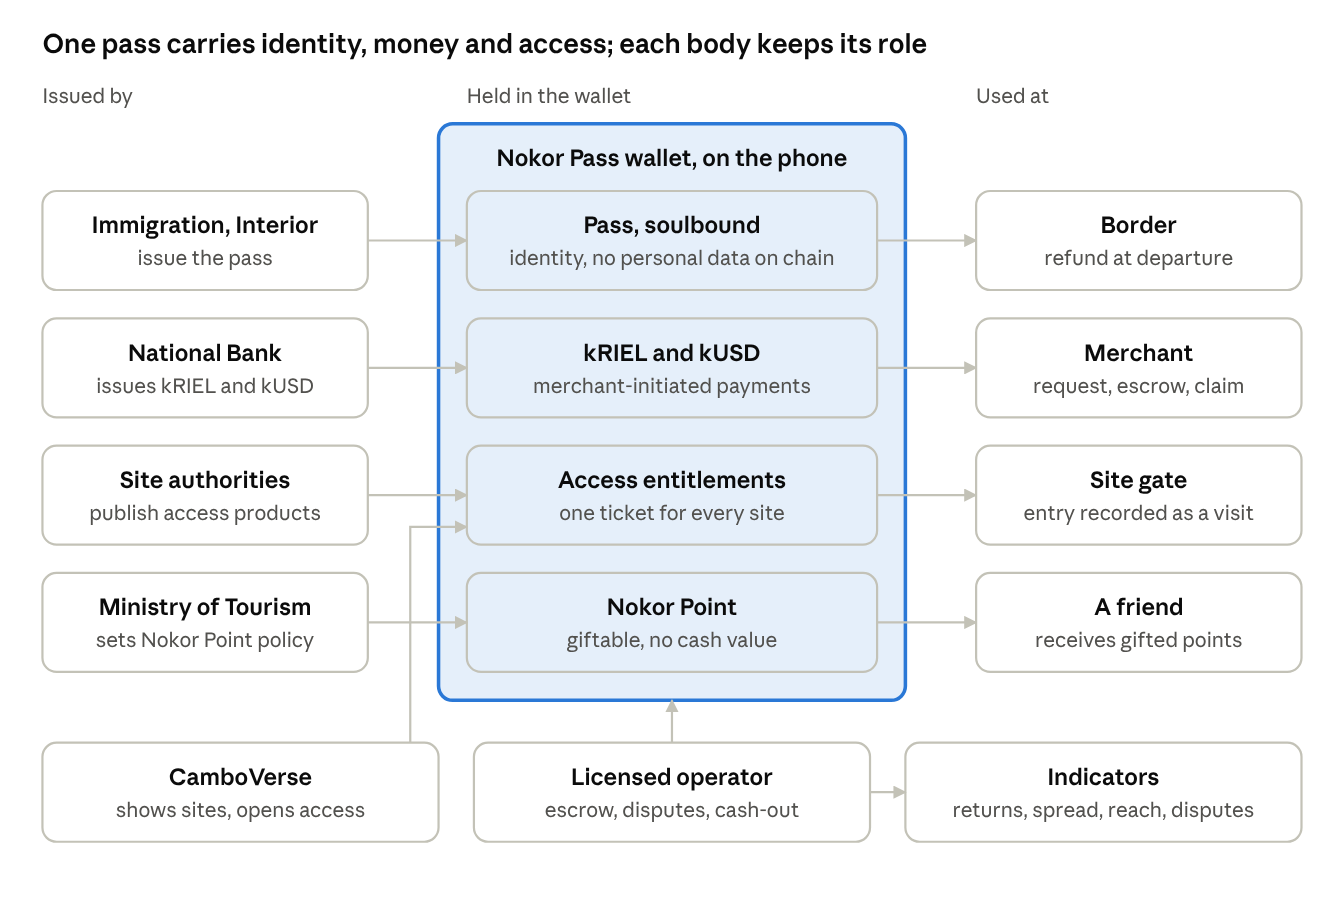
\includegraphics[width=0.86\textwidth]{figures/architecture.png}
  \caption{Nokor Pass architecture. Institutions on the left issue into the
  wallet; what the wallet holds is used at the places on the right. The
  licensed operator runs escrow, disputes and cash-out; CamboVerse links to
  access products; every event feeds the indicators.}
  \label{fig:architecture}
\end{figure*}

\subsection{The pass}

A visitor's pass is issued by immigration at arrival, from the identity checks
already made for the e-Arrival card or visa. A resident's pass is issued
against the national identity card. The pass is soulbound: it cannot be
transferred or sold.

No personal data is written on chain. The pass records its issuer, its category
(visitor or resident) and its validity, plus a keyed hash of the holder's
document number, computed with a secret held only by the issuer. A plain hash
would not do: passport and identity numbers are short enough to guess and
match. With a keyed hash, the issuer can recognise a returning holder without
anyone else being able to learn who they are.

The wallet is created silently with a passkey on the phone. Transaction fees
are paid by the operator through a paymaster, so the holder never holds or sees
the chain's native currency.

\subsection{Payments: kRIEL and kUSD}
\label{sec:payments}

\runin{Why not KHQR.} Cambodia's national QR rail, KHQR, is fast and almost
universal. But as \citet{chay2026qrseal} sets out, it leaves the payer exposed
in ways a visitor cannot see. A sticker can cover a merchant's code. A code can
open a phishing page. A genuine code can be presented with a false story. A
fare agreed in riel can be charged in dollars, as a Phnom Penh driver was
arrested for doing in October 2025. And every transfer is final, into an
account that holds money the receiver can withdraw at once. Signing the codes
closes forgery; it does not close the rest.

\runin{The tokens.} kRIEL and kUSD are fully reserved tokens issued by the
central bank, one for one with riel and dollars. Holders top up by card, by
bank transfer, or with cash at airports, hotels and banks; the exchange rate is
shown once, at top-up.

\runin{Paying.} The payee starts every payment, not the payer. A merchant's
registered device sends a request; the payer's wallet shows the merchant's
registered name, the amount, the currency by its ISO code, and for visitors the
amount in their home currency. The payer approves with the passkey. The payer
never scans a code.

\runin{Escrow and disputes.} An approved payment does not go straight to the
merchant. It sits in escrow for a dispute window, such as 24 hours, and then
releases. Within the window the payer can dispute it, and the operator can
reverse it from escrow. For regulated categories such as tuk-tuks and boats, a
request above the published reference fare for the route is flagged before
approval.

\runin{Cash-out.} A merchant's released balance is a claim, not cash. It
converts to money only through the operator, into the merchant's bank account,
with Bakong as the settlement rail behind the scenes. Exit controls apply by
risk class: new or unusual accounts face delays and limits; established
merchants do not.

\subsection{Site access and departure}

Site authorities publish access products as entitlements: a day at Angkor, a
three-day pass, a bundle of lesser-known sites. Holders buy them with kRIEL or
kUSD, and the entitlement is recorded on the pass. At the gate, the site's
device starts the check and the holder confirms on the phone; the entry is
recorded as a visit.

At departure, a visitor's remaining balance is converted back to their card or
to cash, and the wallet is emptied. The pass remains as the record of the trip.
Residents keep their balance and cash out to their bank at any time.

\subsection{CamboVerse}
\label{sec:camboverse}

CamboVerse is an open-source virtual Cambodia, built at our university as a
digital public good, in which 14 heritage sites can already be walked on an
ordinary phone \citep{chay2026precinct}. Its core holds no money and mints no
tokens; its rules forbid it. In this design it plays one role: it shows people
the sites they would otherwise never hear of, especially those beyond Angkor,
and links each to the access product that opens it. CamboVerse is where
interest starts; Nokor Pass is where it becomes a visit.

\subsection{Nokor Point}

Nokor Point is a separate token. Holders earn it from verified events: a
payment to a registered merchant, an entry at a site gate. It has no guaranteed
cash value and can never be converted into kRIEL or kUSD. What it buys is set
by merchants' offers and by government policy; the state guarantees one small
baseline use, such as a discount on site access, so that points are worth
something even before merchants join.

Points can be given to any other pass holder, and each point carries the time
it was earned. Two uses follow. A visitor can give points to a friend at home,
which makes a recommendation carry something of value. And because each point
records when it was earned, the system can tell when a point earned on one trip
is spent on a later trip, or by someone else.

\subsection{Chain, openness and privacy}

The contracts run on Base, a public Ethereum layer-2 network: the pass, kRIEL
and kUSD with their escrow, freeze and recovery functions, the access
entitlements, and Nokor Point. The specification and contracts are published
as open source, so anyone can check them. Keys, identity data and the issuer's
hashing secret are not published. Because a public ledger shows every balance
and transfer by address, merchants settle through rotating addresses, and no
address is ever linked on chain to a name.

% ---------------------------------------------------------------------------
\section{What Follows}
\label{sec:follows}

The claims in this section are analytic unless marked otherwise: they follow
from the rules in Section~\ref{sec:design}.

\subsection{Fraud the payer can no longer suffer}

Because the payer never scans a code, three attacks that rest on scanning have
nothing to act on. Table~\ref{tab:fraud} uses the problem numbers of
\citet{chay2026qrseal}.

\begin{table*}[t]
  \centering
  \small
  \caption{Payment fraud under KHQR and under Nokor Pass. Problem numbers follow \citet{chay2026qrseal}.}
  \label{tab:fraud}
  \begin{tabularx}{\textwidth}{@{}p{0.27\textwidth}p{0.2\textwidth}L@{}}
    \toprule
    Problem & Under KHQR & Under Nokor Pass \\
    \midrule
    P1 Overlay: a sticker over a merchant's code & Payment goes to a stranger & No code is scanned; the request comes from a registered device \\
    P3 Quishing: a code that opens a phishing page & Credentials or card details stolen & No code is scanned \\
    P9 Currency substitution: riel agreed, dollars charged & The amount is final & Currency shown by ISO code with a home-currency amount; a fare above the reference is flagged; the payment can be disputed from escrow \\
    P4 Genuine payee, false story & Not addressed by signing & Not prevented; reversible within the dispute window if reported in time \\
    P8 Mule cash-out & Funds forwarded in minutes & Proceeds are a claim; cash-out is delayed and limited for new and unusual accounts \\
    \bottomrule
  \end{tabularx}
\end{table*}

Two of these are only partly closed. A false story told to the payer (P4) is
still possible; the design makes it reversible within the window, not
impossible. And the mule exit (P8) is slowed, not stopped.

\subsection{Exit controls bind from the first payment}

In the design of \citet{chay2026qrseal}, the strongest protection against fraud
on a final rail is to remove the liquidity of the proceeds: if what the receiver
holds is a claim redeemable only through a chokepoint, a fraud does not pay
whether or not anyone notices it. Under KHQR that control would have to be
imposed on millions of existing accounts. Under Nokor Pass it is the default:
every merchant balance is a claim from the first payment, and the operator's
rules decide when it becomes money. Screening that depends on someone first
reporting an account protects no one before the report; exit controls do.

\subsection{Repeat visits and word of mouth become measurable}
\label{sec:measure}

Each event in the design leaves a record, so the measures the strategy needs
can be computed directly (Table~\ref{tab:indicators}). None of them requires
knowing who anyone is.

\begin{table}[t]
  \centering
  \small
  \caption{Indicators computed from Nokor Pass events.}
  \label{tab:indicators}
  \begin{tabularx}{\columnwidth}{@{}p{0.3\columnwidth}L@{}}
    \toprule
    Indicator & How it is computed \\
    \midrule
    Repeat-visitor rate & Share of visitor passes issued whose keyed document hash matches an earlier pass \\
    Return value rate & Share of Nokor Points spent on a later trip than the one on which they were earned \\
    Spread rate & Share of Nokor Points spent by a different pass from the one that earned them \\
    Reach beyond Angkor & Site entries outside the Angkor park as a share of all entries, by province \\
    Dispute rate & Disputes per thousand payments, by merchant category and province \\
    Spending by place & kRIEL and kUSD payments by province and sector \\
    \bottomrule
  \end{tabularx}
\end{table}

The repeat-visitor rate measures returns by the same person. The return value
rate and spread rate measure the two forms of word of mouth our argument relies
on: a visitor coming back, and a visitor sending someone else. Today Cambodia
measures arrivals; under this design it would also measure returns.

\subsection{Honesty pays more than cheating}

It follows from the rules that a merchant who overcharges a visitor risks a
reversed payment and a slower cash-out, while a merchant with few disputes is
paid on time. Whether merchants change their behaviour in response is
conjectural. We expect it, because the incentive is immediate and personal, but
we have observed nothing.

% ---------------------------------------------------------------------------
\section{Required Institutional Changes}
\label{sec:institutions}

Without the state, this design is nothing. No university, company or ministry
acting alone can issue an identity at the border, a riel token, or a site
ticket. The design deliberately ignores the rules in force today;
Table~\ref{tab:institutions} names what would have to change, and who would
change it.

\begin{table*}[t]
  \centering
  \small
  \caption{Institutions, what each must do, and what changes. All roles are proposals.}
  \label{tab:institutions}
  \begin{tabularx}{\textwidth}{@{}p{0.22\textwidth}p{0.33\textwidth}L@{}}
    \toprule
    Institution & What it must do & What changes \\
    \midrule
    General Department of Immigration & Issue the pass at arrival from e-Arrival and visa checks & Immigration becomes an issuer of a digital credential, not only a stamp \\
    Ministry of Interior & Issue the pass to residents against the national identity card & The identity system is linked to a pass without putting personal data on chain \\
    National Bank of Cambodia & Issue kRIEL and kUSD, fully reserved; set merchant cash-out rules & The central bank issues tokens on a public chain and licenses an operator as the cash-out chokepoint \\
    Ministry of Tourism & Own the programme; set Nokor Point policy and its baseline use; publish reference fares and site data & Tourism policy is measured by returns and disputes, not only arrivals \\
    Angkor Enterprise and other site authorities & Accept the pass as the site ticket; publish access products & Paper and online tickets give way to entitlements on the pass \\
    A licensed operator & Run escrow, disputes, merchant onboarding, screening and the paymaster & One accountable party holds the chokepoint the design depends on \\
    CamboVerse Center, NUM & Maintain CamboVerse and the open reference implementation & A university builds public rails; private firms build the apps on them \\
    \bottomrule
  \end{tabularx}
\end{table*}

Two principles follow from our own position. The state should build the rails
and leave applications to the private sector: banks, wallets and travel firms
should be free to build Nokor Pass--compatible apps against the open
specification. And the design asks for coordination, not confrontation. It does
not require the state to police drivers, guides or vendors one by one; it
changes what pays, and lets the incentive do the policing.

% ---------------------------------------------------------------------------
\section{What This Does Not Solve}
\label{sec:notsolve}

\runin{The reputation damage itself.} The main cause of the 2026 fall, by the
Ministry's own account, is publicity about scam compounds. That is not a
problem of tourist payments, and no pass changes a headline. Only visible
enforcement against the compounds does. Nokor Pass can make each visit
trustworthy and prove that it was; it cannot persuade someone who has decided
not to come. We regard it as the second half of a strategy whose first half is
enforcement.

\runin{The border, fuel prices and global demand.} These lie outside the
tourism system. The Thai border alone removed most of the overland arrivals
between January and May 2026.

\runin{What happens off the payment rail.} Litter at sites, aggressive touts,
poor roads to remote sites and rude service leave no payment record and cannot
be reversed. The design reveals some of them through disputes and ratings; it
fixes none of them. Someone still has to act on the data.

\runin{Places with no gate and no merchant.} A waterfall, a village walk or a
viewpoint produces no entry and no payment, so it is invisible to the
indicators. These are often exactly the lesser-known places the strategy wants
to open.

\runin{Speed.} A national pass takes years to issue, legislate and adopt. It
addresses the structure of Cambodian tourism, not this year's decline.

\runin{A false story told to the payer.} A merchant who lies about why a
payment is owed still receives a genuine, approved payment. The design makes it
reversible if the payer notices within the window, not impossible.

% ---------------------------------------------------------------------------
\section{What We Do Not Know}
\label{sec:unknown}

\runin{Whether visitors will use it.} The design works only if nearly every
visitor holds a pass. That requires it to be part of the arrival process, not
an optional download. We do not know how visitors will react to a mandatory
wallet, or how many will prefer cash.

\runin{Whether points will be given.} That visitors will give Nokor Points to
friends, and that friends will come because of them, is conjectural. Points
with no guaranteed value may simply be ignored if few merchants honour them.
The baseline use is meant to prevent that; we do not know whether it is enough.

\runin{Whether behaviour will change.} That merchants who face reversals and
slower cash-out will cheat less is a claim about behaviour. We expect it and
have not observed it.

\runin{The cost to small traders.} Exit controls delay money for new accounts.
A market seller who needs today's takings today is exactly who Cambodia's
payment system was built to serve. If the risk classes are drawn badly, honest
newcomers carry the cost.

\runin{Privacy on a public chain.} No personal data is written on chain, but
every balance and transfer is visible by address. If an address is ever linked
to a person, their spending becomes public. Rotating addresses reduce this;
they do not remove it.

\runin{Sovereignty.} Base is operated by a foreign company, Coinbase, which
runs its sequencer. A national pass and national tokens on that network depend
on its continued operation. The contracts can be redeployed on another
compatible chain, and Base offers a route to withdraw through Ethereum itself,
but whether the state accepts that dependence is a political question we
cannot answer.

\runin{Whether the state will act.} Everything above assumes that seven
institutions will change their rules and work together. That is the largest
unknown, and the one this paper can least affect.

% ---------------------------------------------------------------------------
\section{Next Steps}
\label{sec:next}

The work proceeds in a straight run, each step gating the next.

\begin{enumerate}
  \item \textbf{Publish the specification} of the pass, the tokens, escrow and
  disputes, cash-out rules, access entitlements, Nokor Point and the data each
  event records.
  \item \textbf{Build a reference prototype on a Base test network}, as open
  source under the CamboVerse Center: the pass, kRIEL and kUSD with escrow, a
  visitor wallet, a merchant request, a gate check and Nokor Point. Revise this
  paper so that every specified claim matches the prototype.
  \item \textbf{Commission an independent security audit} of the contracts,
  before any real money is involved.
  \item \textbf{Engage the institutions} in Section~\ref{sec:institutions},
  starting with the Ministry of Tourism, the central bank and Angkor
  Enterprise.
  \item \textbf{Pilot in Siem Reap.} About half of all visitors go there,
  complaints concentrate there, and Angkor's gates give a clean access test.
  The pilot would cover site access, tuk-tuks, restaurants and hotels.
  \item \textbf{Judge the pilot after one high season} on the indicators in
  Section~\ref{sec:measure}, against the period before it: the dispute rate,
  the reach beyond Angkor, and early signs of points given and spent.
  \item \textbf{Extend nationally} only if the pilot shows the indicators
  moving, and adjust the risk classes and dispute window from what it shows.
\end{enumerate}

Each step should be read against Section~\ref{sec:notsolve}: the pilot cannot
show whether Cambodia's image recovers, only whether visits inside the system
become more trustworthy and whether returns can be counted.

% ---------------------------------------------------------------------------
\section{Conclusion}
\label{sec:conclusion}

Cambodia does not lack attractions; it lacks belief. A destination whose image
has been damaged cannot advertise its way back, because the people it needs to
reach no longer trust its messages. They trust people who went. The four cases
we read point the same way: Japan's visitors return because of their last
visit, Vietnam grew without a large promotion budget, Singapore's reputation is
the residue of trust, and Colombia's slogan worked only because visitors
confirmed it.

The strategy that follows is to make every visit trustworthy, and to make
returns and recommendations count. Nokor Pass is our instrument for both. It
removes the payment frauds that rest on scanning a code, makes a merchant's
proceeds a claim until a dispute window has passed, opens every site with one
pass, and lets the state measure returns, not only arrivals. Nokor Point turns
a recommendation into something that can be given and counted. CamboVerse shows
people the places they would otherwise never hear of.

None of it works unless the state builds it, and none of it replaces
enforcement against the compounds whose publicity caused the fall. What it
offers is a long-term structure in place of short-term spending: a way for each
good visit to add to the next.

\small
\bibliographystyle{plainnat}
\bibliography{references}

\end{document}
